% HMC Math dept HW template example
% v0.04 by Eric J. Malm, 10 Mar 2005
\documentclass[12pt,letterpaper,boxed,cm]{hmcpset}

% set 1-inch margins in the document
\usepackage[margin=1in]{geometry}
\usepackage{mathtools}
\usepackage{mathrsfs}
% include this if you want to import graphics files with /includegraphics
\usepackage{graphicx}
\usepackage{cases}
\usepackage{hyperref}
\usepackage{siunitx}

% info for header block in upper right hand corner
\name{John Gaskin}
\class{Computer Science 81}
\assignment{Homework 1}
\duedate{1/24/17}

\providecommand{\t}[1]{\text{#1}}
\newcommand{\pn}[1]{\left( #1 \right)}
\newcommand{\abs}[1]{\left| #1 \right|}
\newcommand{\bk}[1]{\left[ #1 \right]}

\begin{document}
\problemlist{1, 2, 3, 4}

\begin{problem}[1]
    [2 points] Carefully diagnose the error or errors in the following two “proofs”:
    \begin{enumerate}
        \item[A.] [1 point] \textbf{Claim: Horses have an infinite number of legs.}\\
        Proof: Horses have an even number of legs: behind they have two legs, and in front they have fore legs, and this totals six legs. But that is certainly an odd number of legs for a horse, and the only number that is both odd and even is infinity. Therefore, horses have an infinite number of legs.
        \item [B.] [1 point] \textbf{Claim: All horses are the same color.}\\
        Proof: We will show that every nonempty collection of horses is monochromatic by induction on the number of horses $k\ge1$ in the collection.
        \begin{itemize}
            \item \textit{Base case:} Obviously, every set containing one horse is monochromatic (is a set of horses all of the same color).
            \item \textit{Inductive case:} Suppose, inductively, that we know every set of $k \ge 1$ horses is monochromatic. We must show that every set of $k+1$ horses is monochromatic. Assume we have an arbitrary set of $k+1$ horses. By the inductive hypothesis, the first $k$ are a set of a single color, and so are the last $k$:
            \begin{center}
                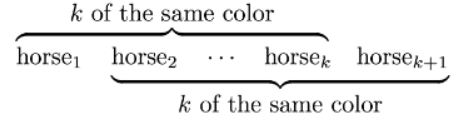
\includegraphics[scale=.7]{01.JPG}
            \end{center}
            Thus, the first and last horse have the same color too, and the entire set of $k+1$ horses is monochromatic.
        \end{itemize}
    \end{enumerate}
\end{problem}

\begin{solution}
    \vfill
\end{solution}
\newpage

\begin{problem}[2]
    [4 points] You might have seen Euclid’s proof that there are an infinite number of primes. Here’s an alternate proof due to Goldbach:\\
    \begin{itemize}
        \item[] Define the Fermat numbers $\displaystyle F_n:=2^{2^n}+1$ for $n=0,1,2\ldots$\\ Then $F_0 = 2^1+1 = 3$ and $F_1 = 2^2+1 = 5$ and $F_2 = 2^4+1 = 17$ and so on.

        \item[] There are infinitely many primes because any two Fermat numbers are relatively prime (have no prime factors in common). So, each successive Fermat number either is a prime we haven’t seen before, or is a product of such primes. \textbf{QED}.\\

        \item[] But how do we know they’re all relatively prime? Well, for every $n\ge1$ one can show that:\\
        \begin{equation}
            \prod_{k=0}^{n-1}F_k=F_n-2
        \end{equation}

        \item[] Thus, if $k$ and $n$ are distinct indices with $0 \le k < n$, and $m$ is any divisor of both $F_k$ and $F_n$ (that is, if $F_k$ is some multiple of $m$, and $F_n$ is some other multiple of $m$), then:
        \begin{align*}
            0&=F_k \bmod m = \pn{\prod  _{k=0}^{n-1}F_k} \bmod m =\pn{F_n-2} \bmod m \\
            &= \pn{F_n \bmod m} - \pn{2 \bmod m} = 0 - \pn{2 \bmod m}
        \end{align*}

        \item[] And if $2 \bmod m = 0$, then 2 is an integer multiple of $m$, which means $m=1$ or 2. \\ But $m=2$ is impossible since all Fermat numbers are odd by their definition. Therefore the only common factor $m$ of $F_k$ and $F_n$ is 1. Since $k$ and $n$ were arbitrary indices, it follows that every pair of distinct Fermat numbers is relatively prime.
    \end{itemize}
    Complete the proof by giving the careful inductive proof that Equation (1) holds for all $n\ge1$.
\end{problem}

\begin{solution}
    \vfill
\end{solution}
\newpage

\begin{problem}[3]
    [13 points] In Hofstadter’s MIU formal system (see the attached description) you start out with one “axiom” and have 4 “rules of inference”.
    \begin{enumerate}
        \item [A.] [4 points] Show that MUIU is a “theorem” of the system (i.e., it can be produced by starting with the axiom MI and applying zero or more rules).
        \item [B.] [4 points] Prove carefully that UM is \textbf{not} a theorem of the system, i.e., not derivable from the axiom by the given rules of inference. (You will want to use structural induction to prove that every derivable “theorem” has some property that UM lacks.)
        \item [C.][5 points] Either show the steps that derive MU in the system, or prove that it is not a theorem (i.e. that no such derivation exists). 
    \end{enumerate}
    \textit{Hint:} We recommend you start by trying to derive MU. If you succeed, you’re done! If not, maybe you can see some pattern in the strings you did derive; if MU doesn’t fit this pattern, that might be inspiration for a proof that MU is not derivable.
\end{problem}

\begin{solution}
    \vfill
\end{solution}
\newpage

\begin{problem}[4]
    [1 easy point] Please wait until you’re done with the rest of the assignment to answer this quick survey:
    \begin{enumerate}
        \item [A.] How long (in hours) did you spend working on this assignment?
        \item [B.] What was the most interesting thing you learned while answering these problems? (We’re sure there was \textit{something} you learned.)
    \end{enumerate}
\end{problem}

\begin{solution}
    \vfill
\end{solution}

% Add pairs of problems and solutions as needed

\end{document}
